\begin{figure*}
\centering
\begin{subfigure}[t]{0.475\textwidth}
\begin{tikzpicture}[thick, scale=0.7, every label/.style={align=left, scale=0.7}]
   \pie[text=legend, sum=auto, hide number, color={blue!60, cyan!60, yellow!60, orange!60}]{
      11/15.7\%,
      29/41.4\%,
      25/35.7\%,
      5/7.1\%
}
\end{tikzpicture}
\caption{Flaws found in \stds{}.}
\label{fig:stdFlawSources}
\end{subfigure}
\hfill
\begin{subfigure}[t]{0.475\textwidth}
\begin{tikzpicture}[thick, scale=0.7, every label/.style={align=left, scale=0.7}]
   \pie[text=legend, sum=auto, hide number, color={blue!60, cyan!60, orange!60, red!60}]{
      19/21.1\%,
      10/11.1\%,
      44/48.9\%,
      17/18.9\%
}
\end{tikzpicture}
\caption{Flaws found in \metas{}.}
\label{fig:metaFlawSources}
\end{subfigure}
\vskip\baselineskip
\begin{subfigure}[t]{0.475\textwidth}
\begin{tikzpicture}[thick, scale=0.7, every label/.style={align=left, scale=0.7}]
   \pie[text=legend, sum=auto, hide number, color={cyan!60, orange!60, red!60, blue!60!cyan!60}]{
      4/6.9\%,
      26/44.8\%,
      14/24.1\%,
      14/24.1\%
}
\end{tikzpicture}
\caption{Flaws found in \texts{}.}
\label{fig:textFlawSources}
\end{subfigure}
\hfill
\begin{subfigure}[t]{0.475\textwidth}
\begin{tikzpicture}[thick, scale=0.7, every label/.style={align=left, scale=0.7}]
   \pie[text=legend, sum=auto, hide number, color={blue!60, cyan!60, orange!60, red!60, blue!60!cyan!60, cyan!60!yellow!60}]{
      10/13\%,
      3/3.9\%,
      23/29.9\%,
      24/31.2\%,
      10/13\%,
      7/9.1\%
}
\end{tikzpicture}
\caption{Flaws found in \papers{}.}
\label{fig:paperFlawSources}
\end{subfigure}
\vskip\baselineskip
\begin{center}
\begin{subfigure}[t]{\linewidth}
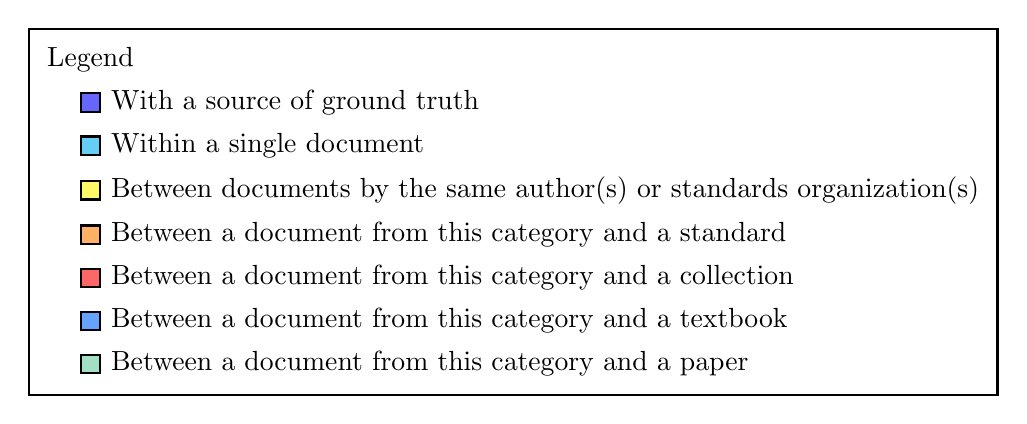
\begin{tikzpicture}
\matrix [thick, draw=black] {
\node[label=center:Legend] {{}}; \\
\node[thick, shape=rectangle, draw=black, fill=blue!60, label=right:{With a source of ground truth}](0) {}; \\
\node[thick, shape=rectangle, draw=black, fill=cyan!60, label=right:{Within a single document}](1) {}; \\
\node[thick, shape=rectangle, draw=black, fill=yellow!60, label=right:{Between documents by the same author(s) or standards organization(s)}](2) {}; \\
\node[thick, shape=rectangle, draw=black, fill=orange!60, label=right:{Between a document from this category and a standard}](3) {}; \\
\node[thick, shape=rectangle, draw=black, fill=red!60, label=right:{Between a document from this category and a collection}](4) {}; \\
\node[thick, shape=rectangle, draw=black, fill=blue!60!cyan!60, label=right:{Between a document from this category and a textbook}](5) {}; \\
\node[thick, shape=rectangle, draw=black, fill=cyan!60!yellow!60, label=right:{Between a document from this category and a paper}](6) {}; \\
};
\end{tikzpicture}
\end{subfigure}
\end{center}
\hfill
\caption{Sources of flaws based on \hyperref[sources]{source tier}.}
\label{fig:flawSources}
\end{figure*}
